\documentclass{article}

\usepackage[T1]{fontenc}
\usepackage{amsmath,amssymb}
\usepackage[paperwidth=29.2cm,paperheight=19.2cm,margin=0.35cm]{geometry}
\usepackage{lmodern}
\usepackage{tikz}
\usetikzlibrary{
  arrows.meta,
  backgrounds,
  calc,
  decorations.pathreplacing,
  fit,
  positioning,
  shapes.geometric
}

\definecolor{navy}{HTML}{17365D}
\definecolor{stateblue}{HTML}{2F75B5}
\definecolor{branchpurple}{HTML}{7030A0}
\definecolor{motionteal}{HTML}{009C9C}
\definecolor{actorange}{HTML}{ED7D31}
\definecolor{safetyred}{HTML}{C00000}
\definecolor{targetgreen}{HTML}{70AD47}
\definecolor{softgray}{HTML}{F2F4F7}
\definecolor{midgray}{HTML}{6B7280}

\tikzset{
  font=\sffamily,
  stage/.style={
    rounded corners=3pt,
    draw=#1,
    fill=#1!6,
    line width=1.1pt,
    text width=6.15cm,
    minimum height=5.25cm,
    inner sep=8pt,
    align=left
  },
  stage/.default=stateblue,
  stage title/.style={font=\bfseries\normalsize, text=#1},
  flow arrow/.style={-{Latex[length=3.2mm,width=2.1mm]}, line width=1.2pt, draw=navy},
  feedback/.style={-{Latex[length=3.2mm,width=2.1mm]}, line width=1.25pt, draw=midgray},
  labelbox/.style={fill=white, inner sep=2pt, font=\scriptsize, text=navy, align=center},
  mode/.style={rounded corners=2pt, draw=navy!70, fill=navy!5, minimum height=0.72cm,
    inner xsep=7pt, font=\bfseries\scriptsize, text=navy},
  exception/.style={rounded corners=2pt, draw=safetyred, fill=safetyred!6,
    inner sep=5pt, font=\scriptsize, text=safetyred, align=center},
  small note/.style={font=\scriptsize, text=midgray, align=left},
  vessel/.style={draw=midgray!65, line width=9pt, line cap=round, line join=round},
  centerline/.style={draw=stateblue, line width=1pt, dashed},
  particle/.style={circle, fill=navy, draw=white, line width=0.5pt, minimum size=5pt, inner sep=0pt},
  coil/.style={draw=actorange, fill=actorange!15, line width=1pt, rounded corners=1pt}
}

\begin{document}
\pagestyle{empty}
\noindent
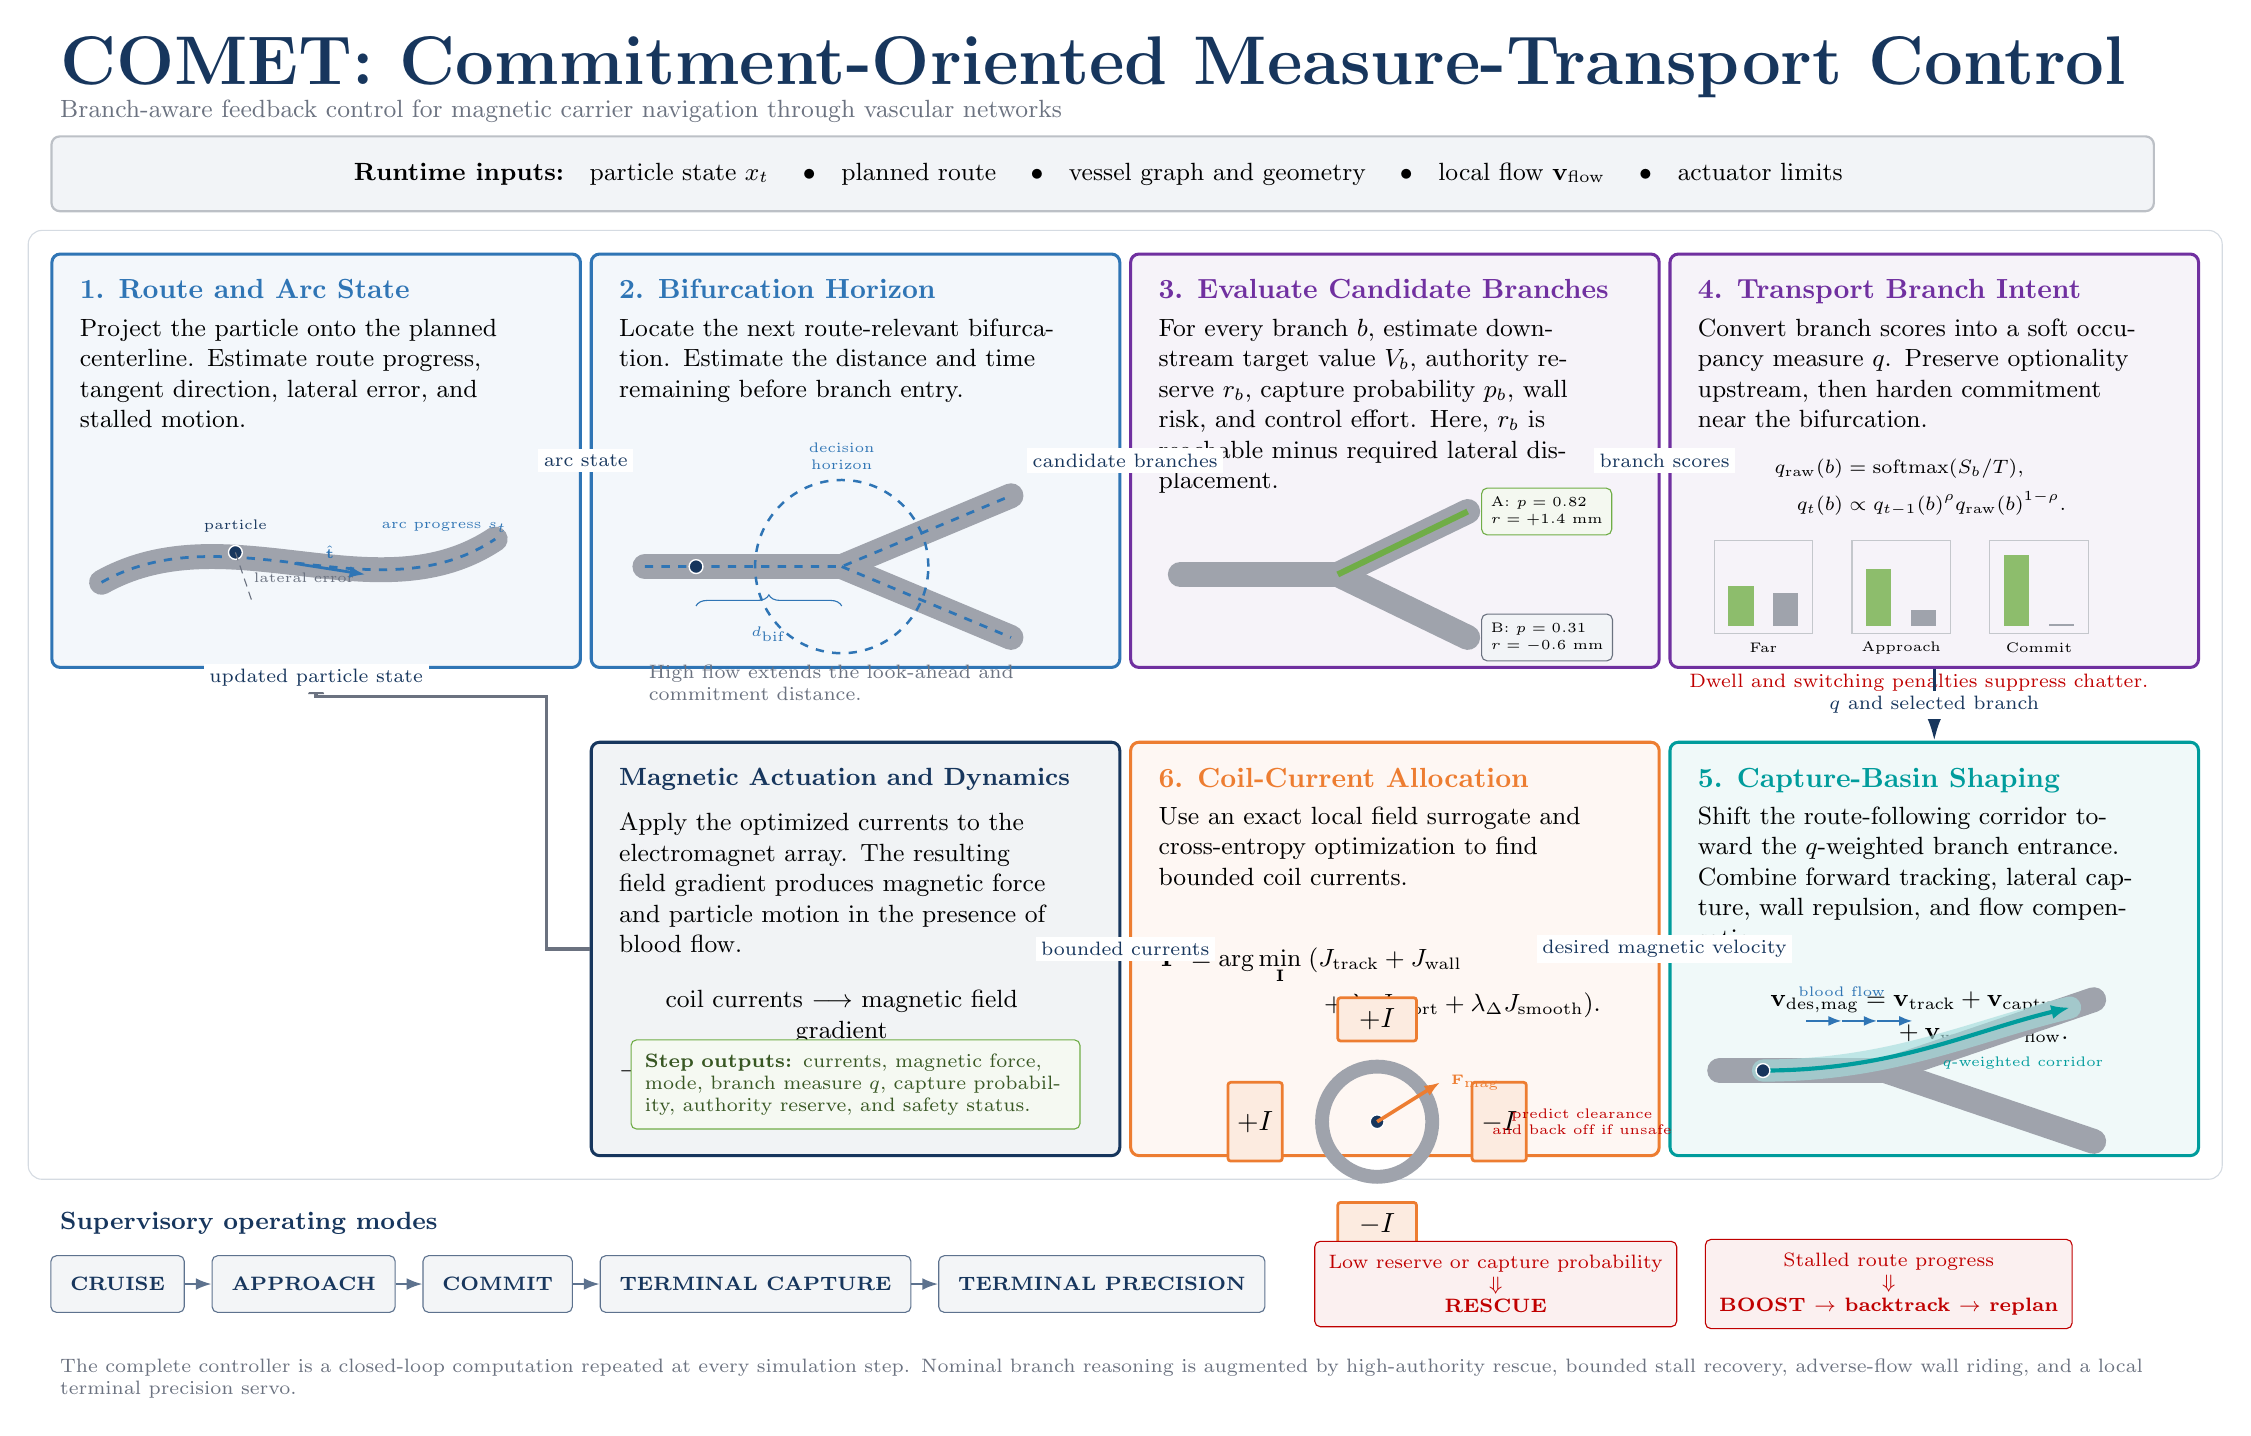
\begin{tikzpicture}[x=1cm,y=1cm]

% ---------------------------------------------------------------------------
% Title and input ribbon
% ---------------------------------------------------------------------------
\node[font=\bfseries\fontsize{23}{26}\selectfont, text=navy, anchor=west]
  (title) at (0,17.6) {COMET: Commitment-Oriented Measure-Transport Control};
\node[font=\small, text=midgray, anchor=west]
  at (0,17.05) {Branch-aware feedback control for magnetic carrier navigation through vascular networks};

\node[rounded corners=3pt, draw=midgray!45, fill=softgray, line width=0.8pt,
      minimum width=26.7cm, minimum height=0.95cm, anchor=west, align=center,
      font=\small] (inputs) at (0,16.25) {
  \textbf{Runtime inputs:}\quad particle state $x_t$ \quad$\bullet$\quad planned route
  \quad$\bullet$\quad vessel graph and geometry \quad$\bullet$\quad
  local flow $\mathbf v_{\mathrm{flow}}$ \quad$\bullet$\quad actuator limits
};

% ---------------------------------------------------------------------------
% Main six-stage pipeline
% ---------------------------------------------------------------------------
\node[stage=stateblue, anchor=north west] (s1) at (0,15.25) {};
\node[stage=stateblue, anchor=north west] (s2) at (6.85,15.25) {};
\node[stage=branchpurple, anchor=north west] (s3) at (13.70,15.25) {};
\node[stage=branchpurple, anchor=north west] (s4) at (20.55,15.25) {};

\node[stage=motionteal, anchor=north west] (s5) at (20.55,9.05) {};
\node[stage=actorange, anchor=north west] (s6) at (13.70,9.05) {};
\node[rounded corners=3pt, draw=navy, fill=navy!6, line width=1.1pt,
      text width=6.15cm, minimum height=5.25cm, inner sep=8pt, align=left,
      anchor=north west] (plant) at (6.85,9.05) {};

% Stage 1 content
\node[stage title=stateblue, anchor=north west] at ($(s1.north west)+(0.25,-0.22)$)
  {1. Route and Arc State};
\node[font=\small, text width=5.65cm, align=left, anchor=north west]
  at ($(s1.north west)+(0.25,-0.72)$) {
  Project the particle onto the planned centerline. Estimate route progress,
  tangent direction, lateral error, and stalled motion.
};
\begin{scope}[shift={($(s1.south west)+(0.65,0.65)$)}]
  \draw[vessel] (0,0.45) .. controls (1.6,1.35) and (3.5,0.0) .. (5.0,1.0);
  \draw[centerline] (0,0.45) .. controls (1.6,1.35) and (3.5,0.0) .. (5.0,1.0);
  \node[particle] (p1) at (1.7,0.83) {};
  \draw[densely dashed, midgray] (p1.center) -- +(0.22,-0.65)
    node[midway, right, font=\tiny] {lateral error};
  \draw[-{Latex[length=2mm]}, stateblue, line width=1pt] (2.45,0.69) -- (3.35,0.55)
    node[midway, above, font=\tiny] {$\hat{\mathbf t}$};
  \node[font=\tiny, text=navy, above=1pt of p1] {particle};
  \node[font=\tiny, text=stateblue] at (4.35,1.15) {arc progress $s_t$};
\end{scope}

% Stage 2 content
\node[stage title=stateblue, anchor=north west] at ($(s2.north west)+(0.25,-0.22)$)
  {2. Bifurcation Horizon};
\node[font=\small, text width=5.65cm, align=left, anchor=north west]
  at ($(s2.north west)+(0.25,-0.72)$) {
  Locate the next route-relevant bifurcation. Estimate the distance and time
  remaining before branch entry.
};
\begin{scope}[shift={($(s2.south west)+(0.7,0.55)$)}]
  \draw[vessel] (0,0.75) -- (2.5,0.75);
  \draw[vessel] (2.5,0.75) -- (4.65,1.65);
  \draw[vessel] (2.5,0.75) -- (4.65,-0.15);
  \draw[centerline] (0,0.75) -- (2.5,0.75) -- (4.65,1.65);
  \draw[centerline] (2.5,0.75) -- (4.65,-0.15);
  \node[particle] (p2) at (0.65,0.75) {};
  \draw[decorate, decoration={brace, amplitude=4pt}, stateblue]
    (0.65,0.25) -- (2.5,0.25) node[midway, below=4pt, font=\tiny] {$d_{\mathrm{bif}}$};
  \draw[stateblue, dashed, line width=0.9pt] (2.5,0.75) circle[radius=1.1];
  \node[font=\tiny, text=stateblue, align=center] at (2.5,2.15) {decision\\horizon};
  \node[small note, text width=4.8cm] at (2.45,-0.72)
    {High flow extends the look-ahead and commitment distance.};
\end{scope}

% Stage 3 content
\node[stage title=branchpurple, anchor=north west] at ($(s3.north west)+(0.25,-0.22)$)
  {3. Evaluate Candidate Branches};
\node[font=\small, text width=5.65cm, align=left, anchor=north west]
  at ($(s3.north west)+(0.25,-0.72)$) {
  For every branch $b$, estimate downstream target value $V_b$, authority
  reserve $r_b$, capture probability $p_b$, wall risk, and control effort.
  Here, $r_b$ is reachable minus required lateral displacement.
};
\begin{scope}[shift={($(s3.south west)+(0.65,0.45)$)}]
  \draw[vessel] (0,0.75) -- (2.0,0.75);
  \draw[vessel] (2.0,0.75) -- (3.65,1.55);
  \draw[vessel] (2.0,0.75) -- (3.65,-0.05);
  \draw[targetgreen, line width=2.2pt] (2.0,0.75) -- (3.65,1.55);
  \node[draw=targetgreen, fill=targetgreen!8, rounded corners=2pt, font=\tiny,
    align=left, anchor=west] at (3.82,1.55) {A: $p=0.82$\\$r=+1.4$ mm};
  \node[draw=midgray, fill=softgray, rounded corners=2pt, font=\tiny,
    align=left, anchor=west] at (3.82,-0.05) {B: $p=0.31$\\$r=-0.6$ mm};
\end{scope}

% Stage 4 content
\node[stage title=branchpurple, anchor=north west] at ($(s4.north west)+(0.25,-0.22)$)
  {4. Transport Branch Intent};
\node[font=\small, text width=5.65cm, align=left, anchor=north west]
  at ($(s4.north west)+(0.25,-0.72)$) {
  Convert branch scores into a soft occupancy measure $q$. Preserve optionality
  upstream, then harden commitment near the bifurcation.

  \vspace{2pt}
  {\scriptsize
  \[
  \begin{aligned}
    q_{\mathrm{raw}}(b)&=\operatorname{softmax}(S_b/T),\\
    q_t(b)&\propto q_{t-1}(b)^\rho q_{\mathrm{raw}}(b)^{1-\rho}.
  \end{aligned}
  \]
  }
};
\begin{scope}[shift={($(s4.south west)+(0.58,0.45)$)}]
  \foreach \x/\a/\b/\lab in {0/0.55/0.45/Far,1.75/0.78/0.22/Approach,3.5/0.98/0.02/Commit} {
    \draw[midgray!40] (\x,0) rectangle +(1.25,1.18);
    \fill[targetgreen!80] (\x+0.18,0.1) rectangle +(0.32,{0.92*\a});
    \fill[midgray!65] (\x+0.75,0.1) rectangle +(0.32,{0.92*\b});
    \node[font=\tiny] at (\x+0.625,-0.18) {\lab};
  }
  \node[small note, text=safetyred] at (2.6,-0.62)
    {Dwell and switching penalties suppress chatter.};
\end{scope}

% Stage 5 content
\node[stage title=motionteal, anchor=north west] at ($(s5.north west)+(0.25,-0.22)$)
  {5. Capture-Basin Shaping};
\node[font=\small, text width=5.65cm, align=left, anchor=north west]
  at ($(s5.north west)+(0.25,-0.72)$) {
  Shift the route-following corridor toward the $q$-weighted branch entrance.
  Combine forward tracking, lateral capture, wall repulsion, and flow compensation.

  \vspace{2pt}
  \[
  \begin{aligned}
    \mathbf v_{\mathrm{des,mag}}={}&\mathbf v_{\mathrm{track}}
    +\mathbf v_{\mathrm{capture}}\\[-2pt]
    &+\mathbf v_{\mathrm{wall}}-\mathbf v_{\mathrm{flow}}.
  \end{aligned}
  \]
};
\begin{scope}[shift={($(s5.south west)+(0.65,0.45)$)}]
  \draw[vessel] (0,0.65) -- (2.1,0.65);
  \draw[vessel] (2.1,0.65) -- (4.75,1.55);
  \draw[vessel] (2.1,0.65) -- (4.75,-0.25);
  \draw[motionteal!35, line width=8pt, opacity=0.65, line cap=round]
    (0.55,0.65) .. controls (2.2,0.65) and (3.2,1.15) .. (4.45,1.45);
  \draw[-{Latex[length=2.4mm]}, motionteal, line width=1.5pt]
    (0.55,0.65) .. controls (2.2,0.65) and (3.2,1.15) .. (4.45,1.45);
  \node[particle] at (0.55,0.65) {};
  \foreach \x in {1.1,1.55,2.0} {
    \draw[-{Latex[length=1.7mm]}, stateblue, line width=0.8pt]
      (\x,1.28) -- +(0.45,0) ;
  }
  \node[font=\tiny, text=stateblue] at (1.55,1.65) {blood flow};
  \node[font=\tiny, text=motionteal] at (3.85,0.75) {$q$-weighted corridor};
\end{scope}

% Stage 6 content
\node[stage title=actorange, anchor=north west] at ($(s6.north west)+(0.25,-0.22)$)
  {6. Coil-Current Allocation};
\node[font=\small, text width=5.65cm, align=left, anchor=north west]
  at ($(s6.north west)+(0.25,-0.72)$) {
  Use an exact local field surrogate and cross-entropy optimization to find
  bounded coil currents.

  \vspace{1pt}
  \[
  \begin{aligned}
    \mathbf I^*=\arg\min_{\mathbf I}\;(&J_{\mathrm{track}}+J_{\mathrm{wall}}\\[-2pt]
      &+\lambda_IJ_{\mathrm{effort}}+\lambda_\Delta J_{\mathrm{smooth}}).
  \end{aligned}
  \]
};
\begin{scope}[shift={($(s6.south west)+(0.7,0.45)$)}]
  \draw[midgray!65, line width=5pt] (2.45,0.0) circle[radius=0.7];
  \node[particle] at (2.45,0.0) {};
  \node[coil, minimum width=0.55cm, minimum height=1.0cm] at (0.9,0.0) {$+I$};
  \node[coil, minimum width=0.55cm, minimum height=1.0cm] at (4.0,0.0) {$-I$};
  \node[coil, minimum width=1.0cm, minimum height=0.55cm] at (2.45,1.3) {$+I$};
  \node[coil, minimum width=1.0cm, minimum height=0.55cm] at (2.45,-1.3) {$-I$};
  \draw[-{Latex[length=2mm]}, actorange, line width=1.3pt] (2.45,0) -- (3.25,0.5)
    node[right, font=\tiny] {$\mathbf F_{\mathrm{mag}}$};
  \node[font=\tiny, text=safetyred, align=center] at (5.05,0.0)
    {predict clearance\\and back off if unsafe};
\end{scope}

% Plant content
\node[font=\bfseries\small, text=navy, anchor=north west]
  at ($(plant.north west)+(0.25,-0.22)$)
  {Magnetic Actuation and Dynamics};
\node[font=\small, text width=5.65cm, align=left, anchor=north west]
  at ($(plant.north west)+(0.25,-0.80)$) {
  Apply the optimized currents to the electromagnet array. The resulting field
  gradient produces magnetic force and particle motion in the presence of blood flow.

  \vspace{9pt}
  \centering
  coil currents $\longrightarrow$ magnetic field gradient\\[3pt]
  $\longrightarrow$ particle force $\longrightarrow$ updated motion
};
\node[rounded corners=2pt, draw=targetgreen, fill=targetgreen!7, text=targetgreen!50!black,
      font=\scriptsize, align=left, text width=5.35cm, inner sep=5pt, anchor=south]
  at ($(plant.south)+(0,0.35)$) {
  \textbf{Step outputs:} currents, magnetic force, mode, branch measure $q$,
  capture probability, authority reserve, and safety status.
};

% ---------------------------------------------------------------------------
% Main arrows
% ---------------------------------------------------------------------------
\draw[flow arrow] (s1.east) -- (s2.west)
  node[labelbox, midway] {arc state};
\draw[flow arrow] (s2.east) -- (s3.west)
  node[labelbox, midway] {candidate branches};
\draw[flow arrow] (s3.east) -- (s4.west)
  node[labelbox, midway] {branch scores};
\draw[flow arrow] (s4.south) -- (s5.north)
  node[labelbox, midway] {$q$ and selected branch};
\draw[flow arrow] (s5.west) -- (s6.east)
  node[labelbox, midway] {desired magnetic velocity};
\draw[flow arrow] (s6.west) -- (plant.east)
  node[labelbox, midway] {bounded currents};

% Feedback loop returns from plant to stage 1.
\draw[feedback] (plant.west) -- ++(-0.55,0) |- ($(s1.south)+(0,-0.35)$) -- (s1.south)
  node[labelbox, pos=0.67] {updated particle state};

% ---------------------------------------------------------------------------
% Supervisory modes
% ---------------------------------------------------------------------------
\node[font=\bfseries\small, text=navy, anchor=west] at (0,2.92)
  {Supervisory operating modes};

\node[mode, anchor=west] (m1) at (0,2.15) {CRUISE};
\node[mode, right=0.34cm of m1] (m2) {APPROACH};
\node[mode, right=0.34cm of m2] (m3) {COMMIT};
\node[mode, right=0.34cm of m3] (m4) {TERMINAL CAPTURE};
\node[mode, right=0.34cm of m4] (m5) {TERMINAL PRECISION};
\foreach \a/\b in {m1/m2,m2/m3,m3/m4,m4/m5}
  \draw[-{Latex[length=2mm]}, navy!70, line width=0.8pt] (\a.east) -- (\b.west);

\node[exception, anchor=west] (rescue) at (16.05,2.15)
  {Low reserve or capture probability\\$\Downarrow$\\\textbf{RESCUE}};
\node[exception, right=0.35cm of rescue] (boost)
  {Stalled route progress\\$\Downarrow$\\\textbf{BOOST $\rightarrow$ backtrack $\rightarrow$ replan}};

\node[font=\scriptsize, text=midgray, anchor=west, text width=26.6cm]
  at (0,0.95) {
  The complete controller is a closed-loop computation repeated at every simulation step.
  Nominal branch reasoning is augmented by high-authority rescue, bounded stall recovery,
  adverse-flow wall riding, and a local terminal precision servo.
};

% Outer grouping label.
\begin{scope}[on background layer]
  \node[draw=navy!18, rounded corners=5pt, inner sep=8pt,
        fit=(s1)(s4)(plant)(s5), fill=white] {};
\end{scope}

\end{tikzpicture}
\end{document}
